% A2: IBGE, PNAD Contínua TIC 2023, informativo de 2024, p. 10--11.
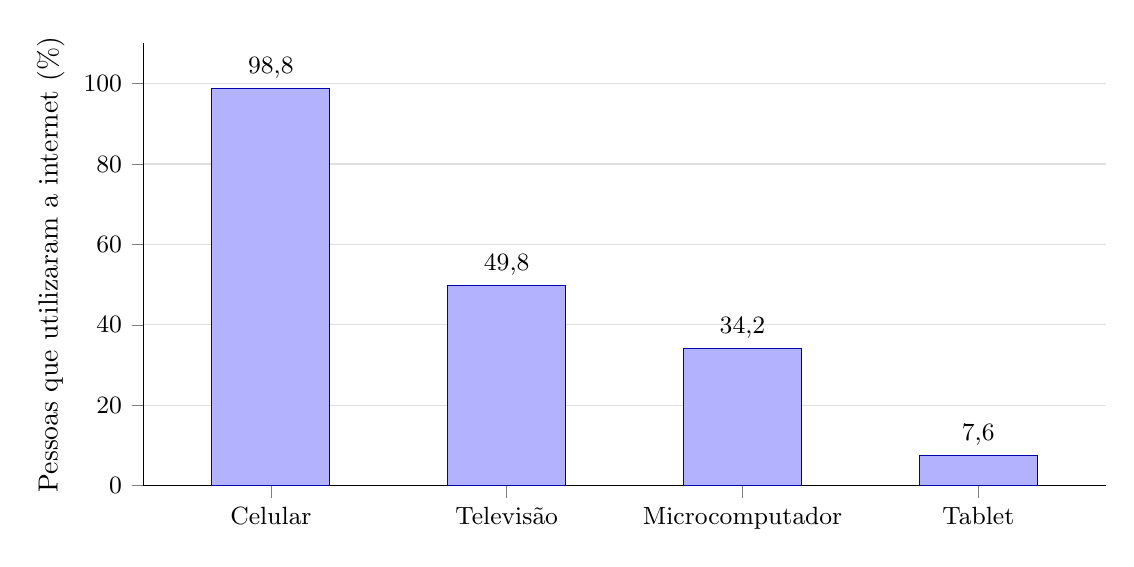
\begin{tikzpicture}
\begin{axis}[
    ybar,bar width=15mm,width=13.8cm,height=7.2cm,
    ymin=0,ymax=110,ytick={0,20,40,60,80,100},
    ylabel={Pessoas que utilizaram a internet (\%)},
    symbolic x coords={Celular,Televisão,Microcomputador,Tablet},
    xtick=data,xticklabel style={font=\small},
    yticklabel style={font=\small},
    nodes near coords,nodes near coords align={vertical},
    every node near coord/.append style={font=\small,
        /pgf/number format/use comma,/pgf/number format/fixed,
        /pgf/number format/precision=1,/pgf/number format/fixed zerofill},
    axis x line*=bottom,axis y line*=left,ymajorgrids=true,
    grid style={black!12},enlarge x limits=0.18,
    tick align=outside,clip=false]
\addplot[draw=blue!65!black,fill=blue!30]
    coordinates {(Celular,98.8) (Televisão,49.8) (Microcomputador,34.2) (Tablet,7.6)};
\end{axis}
\end{tikzpicture}
